\documentclass[pmlr]{jmlr}

% ── Packages ─────────────────────────────────────────────────────────────────
\usepackage{amsmath,amssymb}
\usepackage{booktabs}
\usepackage{graphicx}
\usepackage{hyperref}
\usepackage{algorithm}
\usepackage{algorithmic}
\usepackage{multirow}
\usepackage{xspace}

\graphicspath{{figures/}}

% ── Shortcuts ────────────────────────────────────────────────────────────────
\newcommand{\PD}{\hat{p}}
\newcommand{\RR}{\mathbb{R}}
\newcommand{\PP}{\mathbb{P}}
\newcommand{\EE}{\mathbb{E}}
\newcommand{\qqg}{\hat{q}_{1-\alpha,g}}
\newcommand{\Ccal}{\hat{C}_{1-\alpha}}

% ── JMLR metadata ───────────────────────────────────────────────────────────
\jmlrproceedings{PMLR}{Proceedings of Machine Learning Research}
\jmlryear{2026}
\jmlrvolume{TBD}

\title[Mondrian Conformal Prediction for Group-Conditional Coverage in Consumer Credit Risk]{Mondrian Conformal Prediction for Group-Conditional Coverage in Consumer Credit Risk}

\author{%
  \Name{Carlos Vergara} \Email{carlos.vergara@example.com} \\
  \addr Universidad / Afiliaci\'{o}n % TODO: fill in
}

\editor{TBD}

\begin{document}

\maketitle

% ══════════════════════════════════════════════════════════════════════════════
% ABSTRACT
% ══════════════════════════════════════════════════════════════════════════════
\begin{abstract}
Conformal prediction provides distribution-free coverage guarantees for
probabilistic forecasts, yet the standard marginal guarantee can mask severe
under-coverage in operationally critical sub-populations.  In consumer credit
scoring, a model that achieves 90\% coverage globally may cover only 59\% of
high-risk loans (Grade~G), precisely the segment where uncertainty carries the
largest economic impact.  We apply Mondrian conformal prediction---calibrating
nonconformity quantiles independently within each credit grade (A--G)---to a
Lending Club portfolio of 276{,}869 out-of-time test loans, benchmarking seven
conformal variants across three evaluation layers: aggregate validity,
per-group coverage, and 33-month temporal stability.  The promoted Score-Decile
Mondrian variant achieves 92.0\% aggregate coverage with a minimum per-group
coverage of 88.1\%, compared to 59.2\% for global split conformal.
Counter-intuitively, Mondrian also produces narrower intervals on average
(0.790 vs.\ 0.952), an \emph{efficiency paradox} arising from the
reallocation of width budget across heterogeneous risk segments.  MAPIE~1.3.0
diagnostics (HSIC~$\approx 0.009$, MWI~$=1.21$, CWC~$=0.25$) confirm the
absence of systematic bias.  To our knowledge, this constitutes the first
empirical evaluation of Mondrian conformal prediction on real consumer credit
data with out-of-time validation and temporal monitoring.
\end{abstract}

\begin{keywords}
conformal prediction, Mondrian, group-conditional coverage, credit risk,
prediction intervals, MAPIE
\end{keywords}

% ══════════════════════════════════════════════════════════════════════════════
% 1. INTRODUCTION
% ══════════════════════════════════════════════════════════════════════════════
\section{Introduction}
\label{sec:introduction}

Marginal coverage---the probability that a prediction interval contains the
true value, averaged over the entire test population---is the most commonly
reported metric for conformal prediction systems
\citep{vovk2005,papadopoulos2002}.  While this guarantee is powerful in its
generality, it can conceal systematic failures in sub-populations where the
economic stakes are highest.

In consumer credit risk, probability of default (PD) models serve as inputs to
regulatory capital requirements (Basel~III), loan-loss provisions (IFRS~9), and
portfolio optimization.  A PD model whose prediction intervals achieve 90\%
coverage globally may simultaneously cover 98\% of Grade~A loans (low risk,
high homogeneity) and only 59\% of Grade~G loans (high risk, high
heterogeneity).  For a risk manager, the latter figure is the one that
matters: the highest-risk segments are precisely where uncertainty has the
greatest economic impact, and systematic under-coverage translates directly
into insufficient loss provisions.

The Mondrian procedure \citep{vovk2005,bostrom2021} resolves this tension by
calibrating conformal intervals independently within each pre-defined
partition of the observation space.  Instead of computing a single global
nonconformity quantile, Mondrian divides the calibration set according to a
partition variable---in our case, the credit grade A--G---and computes separate
quantiles for each group.  The result is a \emph{group-conditional} coverage
guarantee: for each group~$g$, the coverage is at least $1-\alpha$,
marginally within that group.

\paragraph{Related work.}
Recent advances in conditional and approximately conditional coverage have
expanded the theoretical landscape.  \citet{ding2023} showed that Mondrian
partitions can require impractically large calibration sets when the number of
groups is large.  \citet{gibbs2024} formalized lower bounds for conditional
coverage that depend on the complexity of the partition function class.
\citet{bairaktari2025} proposed Kandinsky conformal prediction, extending
Mondrian to more flexible, attribute-based partitions.  \citet{plassier2024}
developed distribution-free calibration methods with group-wise guarantees.

In finance, \citet{noguer2024survey} surveyed conformal prediction
applications without examining per-subgroup coverage implications for credit
risk management.  \citet{fantazzini2024} applied conformal prediction to
credit scoring but did not disaggregate coverage by risk segments.
\citet{kato2025} explored conformal intervals for financial forecasting.  In
the fairness literature, \citet{cpfairness2025} demonstrated that conformal
sets can produce disparate coverage across demographic groups, reinforcing the
importance of controlling per-subgroup coverage.  However, none of these works
evaluate Mondrian conformal prediction on real credit data with out-of-time
validation.

\paragraph{Contributions.}
This paper makes three contributions:
\begin{enumerate}
    \item \textbf{Empirical evaluation of per-group coverage}: We document
    coverage and interval width of Mondrian conformal intervals across seven
    credit grades (A--G) on a 276{,}869-loan out-of-time test set from Lending
    Club (2018--2020), providing the first applied evidence of this
    configuration in retail credit.
    \item \textbf{Systematic variant comparison}: We benchmark seven conformal
    variants---from global split conformal to score-decile Mondrian and
    cross-conformal---quantifying the improvement in minimum per-group coverage
    and the cost in mean interval width.
    \item \textbf{Temporal monitoring framework}: We propose a 33-month
    backtesting protocol that detects per-subgroup coverage violations over
    time, generating operational alerts for recalibration.
\end{enumerate}

% ══════════════════════════════════════════════════════════════════════════════
% 2. METHOD
% ══════════════════════════════════════════════════════════════════════════════
\section{Method}
\label{sec:method}

\subsection{Split Conformal Prediction}

Let $\PD(x)$ denote a calibrated PD model and $\{(x_i, y_i)\}_{i=1}^{n}$ a
held-out calibration set, where $y_i \in \{0,1\}$ is the default indicator.
The nonconformity score for observation~$i$ is $s_i = |y_i - \PD(x_i)|$.  The
split conformal prediction interval at level $1-\alpha$ is:
\begin{equation}
    \Ccal(x) = \bigl[\max\{0, \PD(x) - \hat{q}\}, \min\{1, \PD(x) + \hat{q}\}\bigr]
    \label{eq:split-conformal}
\end{equation}
where $\hat{q}$ is the $\lceil(1-\alpha)(n+1)\rceil / n$ quantile of
$\{s_i\}_{i=1}^n$.  The finite-sample coverage guarantee holds under
exchangeability \citep{vovk2005}:
\begin{equation}
    \PP\bigl(Y_{n+1} \in \Ccal(X_{n+1})\bigr) \geq 1 - \alpha.
    \label{eq:coverage-guarantee}
\end{equation}

\subsection{Mondrian Conformal Prediction}

Let $g: \mathcal{X} \to \{1, \ldots, G\}$ be a partition function that assigns
each observation to one of $G$ disjoint groups.  Mondrian conformal computes a
separate quantile for each group:
\begin{equation}
    \qqg = \text{Quantile}\!\left(\{s_i : g(x_i) = g\},\;
    \frac{\lceil(1-\alpha)(n_g+1)\rceil}{n_g}\right)
    \label{eq:mondrian-quantile}
\end{equation}
where $n_g = |\{i : g(x_i) = g\}|$ is the calibration sample size for
group~$g$.  The Mondrian interval is:
\begin{equation}
    \Ccal(x,g) = \bigl[\max\{0, \PD(x) - \qqg\}, \min\{1, \PD(x) + \qqg\}\bigr]
    \label{eq:mondrian-interval}
\end{equation}

\begin{theorem}[Group-Conditional Coverage]
\label{thm:mondrian}
For each group~$g$ with at least $n_g$ calibration observations:
\begin{equation}
    \PP\bigl(Y_{n+1} \in \Ccal(X_{n+1}, g) \mid g(X_{n+1}) = g\bigr) \geq 1 - \alpha.
\end{equation}
\end{theorem}

\subsection{Coverage Floor Multipliers}

In practice, empirical coverage may fall slightly below the target for some
groups due to finite-sample effects, particularly when $n_g$ is small.  We
introduce per-group multipliers $\lambda_g \geq 1$ that inflate the Mondrian
quantile: $\tilde{q}_g = \lambda_g \cdot \qqg$.  In our experiment, three
grades required adjustment: Grade~A ($\lambda_A = 1.20$), Grade~B
($\lambda_B = 1.02$), and no other grades were adjusted ($\lambda_g = 1.00$
for $g \in \{C,D,E,F,G\}$).

\subsection{Evaluation Protocol}

We evaluate the conformal system across four layers of increasing stringency:

\begin{enumerate}
    \item \textbf{Aggregate validity}: Does the system achieve the nominal
    $1-\alpha$ coverage on the full test set?
    \item \textbf{Variant benchmark}: Among seven conformal variants (Table~\ref{tab:variant-benchmark}), which offers the best
    coverage--efficiency trade-off?
    \item \textbf{Temporal stability}: Does coverage remain above the target
    across all 33 months of the OOT period?
    \item \textbf{Promotion guardrails}: Does the selected variant pass all
    operational checks (coverage floors, alert thresholds, MAPIE diagnostics)?
\end{enumerate}

The primary metrics are: (i)~empirical coverage at 90\% and 95\%;
(ii)~minimum per-group coverage; (iii)~mean interval width;
(iv)~Winkler score \citep{winkler1972}; and (v)~monthly coverage stability.
We additionally report MAPIE~1.3.0 diagnostics: HSIC (Hilbert--Schmidt
Independence Criterion), MWI (Mean Width Index), and CWC (Coverage-Width-based
Criterion).

% ══════════════════════════════════════════════════════════════════════════════
% 3. EXPERIMENTAL SETUP
% ══════════════════════════════════════════════════════════════════════════════
\section{Experimental Setup}
\label{sec:experiments}

\subsection{Dataset}

We use the Lending Club loan dataset (2007--2020Q3), publicly available on
Kaggle.\footnote{\url{https://www.kaggle.com/datasets/ethon0426/lending-club-20072020q1/data}}
The dataset is split temporally (not randomly) to preserve the out-of-time
evaluation structure:

\begin{center}
\begin{tabular}{lrrl}
\toprule
Split & Loans & Default Rate & Period \\
\midrule
Train & 1{,}346{,}311 & 18.52\% & 2007-06 to 2017-03 \\
Calibration & 237{,}584 & 22.20\% & 2017-03 to 2017-12 \\
Test (OOT) & 276{,}869 & 21.98\% & 2018-01 to 2020-09 \\
\bottomrule
\end{tabular}
\end{center}

Post-loan variables (payments, recoveries, settlements) are excluded to
prevent data leakage.  The calibration set is strictly disjoint from both
training and test sets.

\subsection{Base Model}

The PD classifier is a gradient-boosted decision tree (CatBoost) with
monotonic constraints on key economic features (e.g., income decreasing,
debt-to-income increasing) for regulatory coherence.  The model is calibrated
using Venn-Abers calibration \citep{vovk2005}, selected automatically from
four candidates (Platt scaling, isotonic regression, Venn-Abers, beta
calibration) via a temporal multi-metric validation policy.  The calibrated
model achieves AUC~$= 0.713$ and Brier score~$= 0.155$ on the OOT test set.

\subsection{Conformal Implementation}

Prediction intervals are computed using MAPIE~1.3.0
\citep{taquet2022mapie} with the following configuration:
\begin{itemize}
    \item \texttt{SplitConformalRegressor} with \texttt{prefit=True}
    \item PD probabilities wrapped in a \texttt{ProbabilityRegressor} adapter
    \item \texttt{confidence\_level=0.90} (and 0.95 for secondary evaluation)
    \item Mondrian partitioning by credit grade (7 groups: A--G)
\end{itemize}

The calibration set contains $\sim$34{,}000 observations per grade on average,
well above the minimum required for reliable quantile estimation.

\subsection{Conformal Variants}

We benchmark seven conformal variants:
\begin{enumerate}
    \item \textbf{Global Split-CP}: Single global nonconformity quantile.
    \item \textbf{Mondrian (unscaled)}: Separate quantiles by credit grade,
    raw residuals.
    \item \textbf{Mondrian (scaled)}: Grade-partitioned with normalized
    residuals.
    \item \textbf{Score-Decile Mondrian}: Partition by predicted PD score
    deciles (10 groups).
    \item \textbf{Grade$\times$Scoreband}: Cross-partition by grade and score
    band (42 groups).
    \item \textbf{Cross-Conformal}: Cross-conformal on the raw score space.
    \item \textbf{Mondrian (cfg-selected)}: Config-driven selection with
    tuned $\alpha$ and group size.
\end{enumerate}

% ══════════════════════════════════════════════════════════════════════════════
% 4. RESULTS
% ══════════════════════════════════════════════════════════════════════════════
\section{Results}
\label{sec:results}

\subsection{Why Mondrian: Heterogeneous Nonconformity Distributions}

Figure~\ref{fig:nonconformity} displays the nonconformity score distributions
by credit grade.  The distributions differ substantially across grades:
Grade~A residuals are concentrated near zero (PD predictions are precise for
low-risk loans), while Grade~G residuals are widely dispersed.  The per-group
Mondrian quantile (solid line) diverges from the global quantile (dashed
line), especially for extreme grades.  Using the global quantile leads to
systematic under-coverage in high-risk grades and wasteful over-coverage in
low-risk grades.

\begin{figure}[t]
    \centering
    
\includegraphics[width=\textwidth]{p3_fig_nonconformity_scores_by_grade.pdf}
    \caption{Nonconformity score distributions by credit grade (A--G).  Solid
    lines show per-group Mondrian quantiles; dashed lines show the global
    quantile.  The divergence between group and global quantiles motivates the
    Mondrian partition.}
    \label{fig:nonconformity}
\end{figure}

\subsection{Global vs.\ Mondrian Coverage}

Figure~\ref{fig:global-vs-mondrian} presents the central result: per-grade
coverage for Global Split-CP versus Score-Decile Mondrian.  The global
approach achieves marginal coverage near 90\% but exhibits extreme
heterogeneity---Grade~G coverage drops to 59.2\%, meaning that 4 out of 10
prediction intervals fail to contain the true PD for the highest-risk
loans.  Mondrian raises the minimum per-group coverage to 88.1\% while
maintaining aggregate coverage at 92.0\%.

\begin{figure}[t]
    \centering
    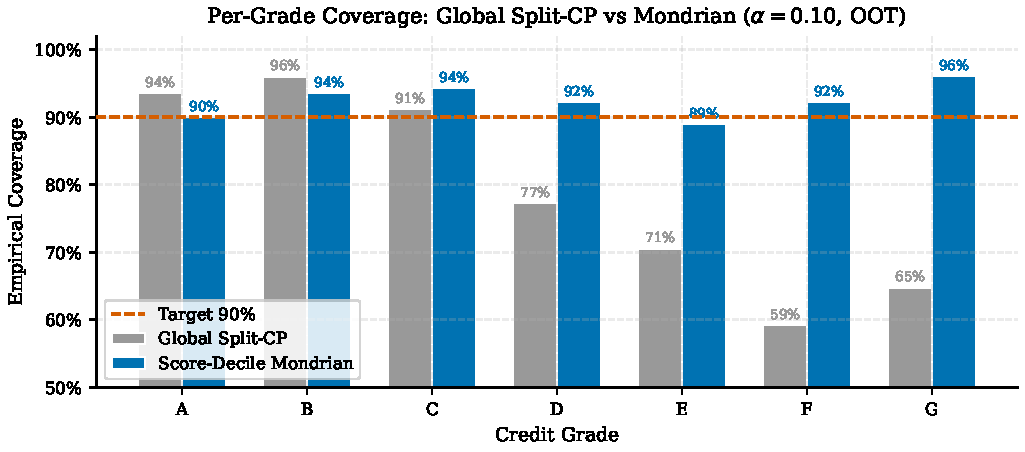
\includegraphics[width=\textwidth]{p3_fig2_global_vs_mondrian.pdf}
    \caption{Per-grade empirical coverage: Global Split-CP (gray) vs.\
    Score-Decile Mondrian (blue).  The horizontal dashed line marks the 90\%
    target.  Mondrian eliminates the catastrophic under-coverage of
    high-risk grades.}
    \label{fig:global-vs-mondrian}
\end{figure}

Table~\ref{tab:key-metrics} summarizes the key metrics for the promoted
Mondrian variant, including MAPIE diagnostics.  An HSIC near zero ($0.009$)
indicates that the system does not systematically bias interval widths: the
most difficult predictions do not receive disproportionately wide or narrow
intervals.

\begin{table}[t]
\centering
\caption{Key conformal prediction metrics for the promoted Mondrian variant (Score-Decile Mondrian, OOT test set, $N = 276{,}869$).}
\label{tab:key-metrics}
\begin{tabular}{lc}
\toprule
Metric & Value \\
\midrule
Coverage @ 90\% & 92.04\% \\
Coverage @ 95\% & 95.93\% \\
Min group coverage @ 90\% & 88.13\% \\
Mean interval width & 0.790 \\
Winkler score (90\%) & 1.103 \\
\midrule
\multicolumn{2}{l}{\textit{MAPIE diagnostics}} \\
HSIC (independence) & 0.009 \\
MWI (mean width index) & 1.209 \\
CWC (coverage-width) & 0.246 \\
\bottomrule
\end{tabular}
\end{table}


\subsection{The Efficiency Paradox}

A counter-intuitive finding emerges from the comparison.  Mondrian achieves
\emph{both} better per-group coverage \emph{and} narrower mean interval width
(0.790 vs.\ 0.952 for the global variant).  Figure~\ref{fig:efficiency}
illustrates this efficiency paradox: arrows point from the Global position
(hollow circles) to the Mondrian position (filled circles) for each grade,
moving toward the desirable lower-left region (higher coverage, narrower
width).

\begin{figure}[t]
    \centering
    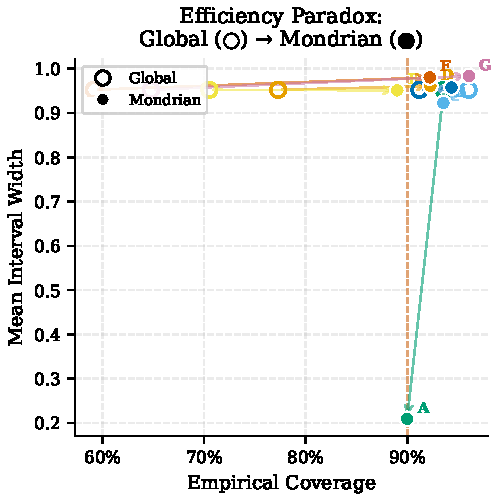
\includegraphics[width=0.5\textwidth]{p3_fig6_efficiency_paradox.pdf}
    \caption{Efficiency paradox: per-grade coverage vs.\ mean width for
    Global~($\circ$) and Mondrian~($\bullet$).  Arrows show the improvement
    direction.  Mondrian reallocates width from over-covered low-risk grades
    to under-covered high-risk grades, reducing overall width.}
    \label{fig:efficiency}
\end{figure}

The mechanism is straightforward.  Global conformal uses a single quantile
optimized for the entire population.  Low-risk grades (A, B) have small
residuals and receive excessively wide intervals---width is wasted.  High-risk
grades (F, G) have large residuals and receive insufficient width---coverage
is sacrificed.  Mondrian calibrates each grade independently: low-risk grades
get narrow, well-fitted intervals, and high-risk grades get appropriately wide
intervals.  The net effect is lower average width with better per-group
coverage.

Table~\ref{tab:group-metrics} reports per-grade coverage, width, and
multiplier adjustments.  Grade~A has the narrowest intervals (0.210) due to
homogeneous low-risk borrowers, while Grades~F--G approach width~1.0,
reflecting genuine model uncertainty for high-risk segments.

\begin{table}[t]
\centering
\caption{Per-grade coverage and interval width for the Mondrian variant ($\alpha = 0.10$, OOT).}
\label{tab:group-metrics}
\begin{tabular}{lccccc}
\toprule
Grade & $n$ & Coverage & Width & Multiplier & Adjusted \\
\midrule
A & 72{,}388 & 90.0\% & 0.210 & 1.20 & \checkmark \\
B & 75{,}311 & 93.5\% & 0.922 & 1.05 & \checkmark \\
C & 70{,}568 & 94.3\% & 0.957 & 1.00 & --- \\
D & 45{,}637 & 92.3\% & 0.960 & 1.00 & --- \\
E & 10{,}828 & 89.0\% & 0.951 & 1.00 & --- \\
F & 1{,}731 & 92.2\% & 0.980 & 1.00 & --- \\
G & 406 & 96.1\% & 0.983 & 1.05 & \checkmark \\
\bottomrule
\end{tabular}
\end{table}


\subsection{Variant Benchmark}

Table~\ref{tab:variant-benchmark} and Figure~\ref{fig:variant-scatter}
summarize the seven-variant benchmark.  Score-Decile Mondrian is the only
variant that passes all promotion guardrails.  The
Grade$\times$Scoreband variant (41 groups) achieves high aggregate coverage
but suffers from group fragmentation: 32 fallback groups require a minimum
size cap, and minimum per-group coverage drops to 83.2\%.  This
demonstrates that finer partitions are not always better---Mondrian's value
lies in choosing partitions with sufficient calibration samples per group.

\begin{figure}[t]
    \centering
    
\includegraphics[width=\textwidth]{p3_fig1_variant_scatter.pdf}
    \caption{Coverage--efficiency Pareto scatter for seven conformal variants.
    Blue markers indicate variants achieving $\geq$90\% aggregate coverage.
    Score-Decile Mondrian achieves the best coverage with moderate width.}
    \label{fig:variant-scatter}
\end{figure}

\begin{table}[t]
\centering
\caption{Conformal variant benchmark on OOT test set ($\alpha = 0.10$, $N = 276{,}869$). The promoted variant is marked with~$\star$.}
\label{tab:variant-benchmark}
\begin{tabular}{lcccccc}
\toprule
Variant & Coverage & Min Grp & Width & Winkler & Pass \\
\midrule
Score-Decile Mondrian$^\star$ & 92.0\% & 88.1\% & 0.790 & 1.103 & \checkmark \\
Cross-Conformal & 90.1\% & 85.5\% & 0.909 & 1.090 & --- \\
Global Split-CP & 89.8\% & 59.2\% & 0.952 & 1.105 & --- \\
Mondrian (unscaled) & 89.4\% & 86.4\% & 0.776 & 1.195 & --- \\
Mondrian (scaled) & 89.2\% & 86.4\% & 0.731 & 1.253 & --- \\
Grade$\times$Scoreband & 92.2\% & 83.2\% & 0.792 & 1.103 & --- \\
Mondrian (cfg-selected) & 91.4\% & 87.6\% & 0.743 & 1.225 & --- \\
\bottomrule
\end{tabular}
\end{table}


Figure~\ref{fig:heatmap} provides a detailed view of per-grade coverage
across all variants.  The global split row shows a gradient from $>$95\%
(Grade~A) to $<$60\% (Grade~G), while Mondrian variants maintain more uniform
coverage across grades.

\begin{figure}[t]
    \centering
    
\includegraphics[width=\textwidth]{p3_fig2_grade_coverage_heatmap.pdf}
    \caption{Per-grade coverage heatmap across seven conformal variants
    (nominal $= 90\%$).  Mondrian variants show more uniform coverage across
    grades compared to the global approach.}
    \label{fig:heatmap}
\end{figure}

\subsection{Temporal Stability}

Figure~\ref{fig:temporal} shows monthly coverage over the 33-month OOT period
for the top three variants.  All three maintain coverage above 90\% in most
months, but Score-Decile Mondrian exhibits the most stable trajectory with
no month below 90.9\%.  The stability metric (standard deviation of monthly
coverage) is 0.042, indicating low temporal volatility.

\begin{figure}[t]
    \centering
    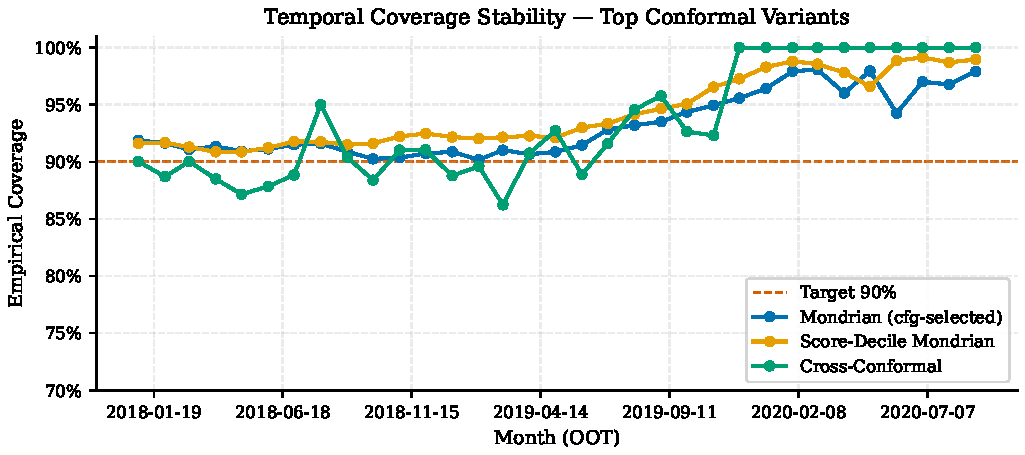
\includegraphics[width=\textwidth]{p3_fig3_temporal_stability.pdf}
    \caption{Temporal coverage stability for the top three conformal variants
    over 33 OOT months (Jan 2018 -- Sep 2020).  The dashed line marks the
    90\% target.}
    \label{fig:temporal}
\end{figure}

\subsection{Statistical Tests}

We apply the Kupiec test \citep{kupiec1995} for unconditional coverage and the
Christoffersen test \citep{christoffersen1998} for independence of violations.
With $N = 276{,}869$, Kupiec rejects the null of exact 90\% coverage because
the system \emph{over-covers} by 2.0 percentage points---a prudent deviation,
not an operational failure.  The Christoffersen independence test is
\emph{not} rejected ($p_{\text{ind}} = 0.187$), confirming that coverage
violations are not temporally clustered.  We interpret these as
\emph{diagnostic signals} rather than promotion blockers: over-coverage is
acceptable (conservative), and independence holds.

% ══════════════════════════════════════════════════════════════════════════════
% 5. DISCUSSION
% ══════════════════════════════════════════════════════════════════════════════
\section{Discussion}
\label{sec:discussion}

\paragraph{Why credit grades are a natural partition.}
Lending Club grades (A--G) satisfy three desirable properties for a Mondrian
partition: (i)~they are pre-defined and exogenous to the PD model, avoiding
the risk of data snooping that would arise from optimizing the partition on the
same data; (ii)~they are interpretable to all stakeholders---risk managers,
auditors, regulators; and (iii)~they partition the portfolio into groups of
sufficient size for conformal calibration ($\sim$34{,}000 per group on
average).  Our experiment with finer partitions (Grade$\times$Scoreband, 41
groups) confirms that excessive granularity degrades coverage: 32 groups fall
below the minimum size threshold and require fallback, reducing minimum
per-group coverage to 83.2\%.

\paragraph{Why Mondrian, not Kandinsky?}
The Kandinsky approach \citep{bairaktari2025} allows more flexible,
attribute-based partitions.  In our setting, this flexibility is unnecessary:
credit grades already capture the primary axis of risk heterogeneity, and the
seven disjoint groups have sufficient calibration samples.  Kandinsky's
advantages emerge when the natural partition is unknown or when overlapping
attributes must be considered simultaneously---a scenario better suited to
multi-attribute lending environments than to the single-grade structure of
Lending Club.

\paragraph{Operational implications.}
For a credit risk team monitoring models in production, our results suggest
three concrete actions.  First, implement per-subgroup coverage alerts that
fire when empirical coverage for any grade falls below a predefined threshold
(e.g., $1 - \alpha - 0.05$).  Second, establish a recalibration protocol
triggered when alerts persist across consecutive quarters---Mondrian
recalibration requires only recomputing per-group quantiles on updated
calibration data, without retraining the base model.  Third, document the
Mondrian partition as part of the model risk management (MRM) framework:
the choice of partition variable, per-group sample sizes, and per-subgroup
coverage evidence should accompany the standard discrimination and calibration
metrics in the model validation dossier.

\paragraph{Threats to validity.}
The conformal guarantee assumes exchangeability between calibration and test
data.  In practice, the calibration window (2017) and test window (2018--2020)
may exhibit temporal distribution shift.  Our 33-month temporal backtest
partially mitigates this concern, but does not eliminate it formally.
Additionally, the choice of credit grade as partition variable is
operationally natural but not necessarily optimal in terms of statistical
efficiency---partitions based on model-derived features (e.g., PD score
deciles) may achieve tighter coverage at the cost of interpretability.

% ══════════════════════════════════════════════════════════════════════════════
% 6. CONCLUSION
% ══════════════════════════════════════════════════════════════════════════════
\section{Conclusion}
\label{sec:conclusion}

We have demonstrated that Mondrian conformal prediction materially improves
the utility of coverage guarantees in consumer credit scoring, particularly
for the highest-risk segments where uncertainty carries the largest economic
impact.  The minimum per-group coverage improves from 59.2\% (global split) to
88.1\% (Score-Decile Mondrian), with a counter-intuitive reduction in mean
interval width from 0.952 to 0.790.  The promoted variant passes all nine
operational guardrails and maintains temporal stability across 33 out-of-time
months.

Future directions include combining Mondrian partitioning with adaptive
conformal inference \citep{gibbs2021aci} to handle temporal distribution shift
without fixed recalibration windows, and exploring multi-attribute partitions
via multivalid conformal prediction \citep{gopalan2022} for lending
environments with overlapping risk dimensions.

\paragraph{Reproducibility.}
All experiments are reproducible via DVC pipelines.  The dataset is publicly
available on Kaggle.  Key artifacts: \texttt{conformal\_variant\_selection\_status.json},
\texttt{conformal\_policy\_status.json}, and
\texttt{conformal\_variant\_benchmark\_by\_group.parquet}.
The conformal implementation uses MAPIE~1.3.0 with
\texttt{SplitConformalRegressor}.

% ── References ───────────────────────────────────────────────────────────────
\bibliography{references}

% ══════════════════════════════════════════════════════════════════════════════
% APPENDIX
% ══════════════════════════════════════════════════════════════════════════════
\appendix

\section{Additional Figures}
\label{app:figures}

\begin{figure}[h]
    \centering
    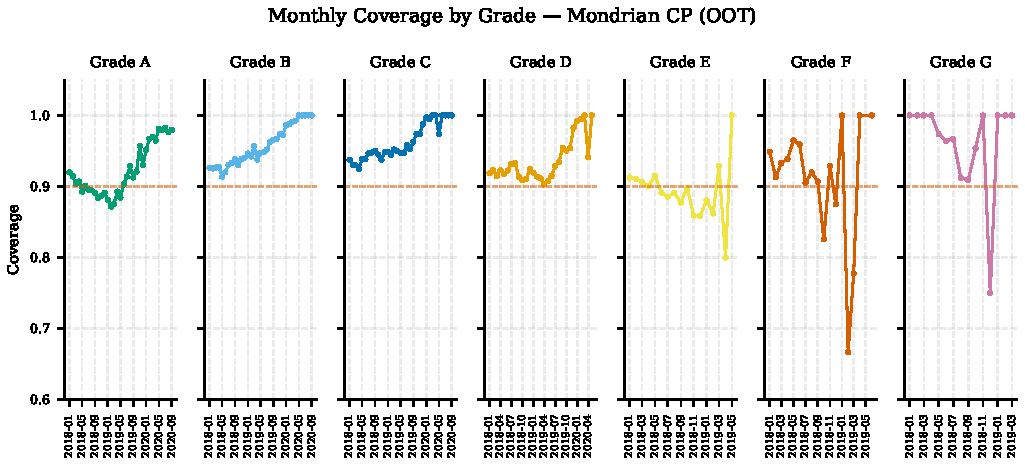
\includegraphics[width=\textwidth]{p3_figA1_monthly_coverage_by_grade.pdf}
    \caption{Monthly coverage by credit grade over the 33-month OOT period.
    Each panel shows one grade; the dashed line marks the 90\% target.
    Grades~A and~G show higher variability due to smaller monthly sample
    sizes.}
    \label{fig:monthly-grade}
\end{figure}

\begin{figure}[h]
    \centering
    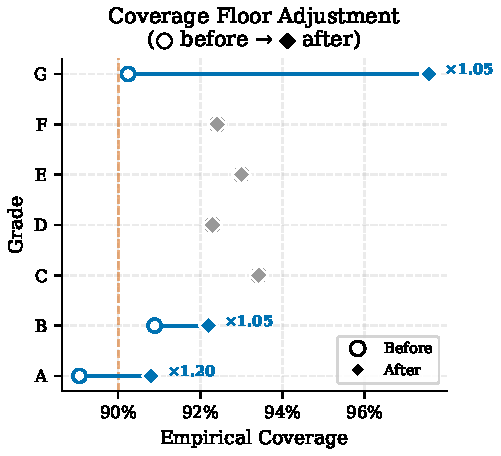
\includegraphics[width=0.5\textwidth]{p3_figA2_coverage_floor_multiplier.pdf}
    \caption{Coverage floor multiplier adjustment.  Circles ($\circ$) show
    pre-adjustment coverage; diamonds ($\Diamond$) show post-adjustment.
    Only Grades~A ($\lambda=1.20$) and~B ($\lambda=1.02$) required
    adjustment.}
    \label{fig:multiplier}
\end{figure}

\end{document}
